\documentclass[10pt]{report}
\usepackage{geometry} 
\usepackage{indentfirst}
\usepackage{hyperref}
\usepackage{color}
\usepackage{comment}
\usepackage[pdftex]{graphicx}  
\usepackage{caption}
\usepackage{natbib}
\usepackage{mathtools}
\usepackage{units}
\usepackage{booktabs}
\usepackage{authblk}
\renewcommand{\baselinestretch}{1.5}
\geometry{a4paper} 
\bibliographystyle{apalike}


%----------------------------------------
%AUTHORS
%----------------------------------------
\title{SUMAC: Supermatrix Constructor version 2.0 Manual}
\author{William A. Freyman\thanks{freyman@berkeley.edu}}
\affil{Department of Integrative Biology, University of California, Berkeley}

\date{}

%-----------------------------------------------------------------------------------------------------------------
% BEGIN DOCUMENT
%-----------------------------------------------------------------------------------------------------------------
\begin{document}
\maketitle

\tableofcontents

%----------------------------------------
% INTRODUCTION
%----------------------------------------

\chapter{Introduction}

\section{About SUMAC}

SUMAC (Supermatrix Constructor) is a Python package to 
data-mine GenBank, construct phylogenetic supermatrices, and assess the phylogenetic decisiveness of a matrix given the pattern of missing sequence data.
It is designed to be run as a command-line program, though
the modules can also be imported and used in other Python scripts.
SUMAC will assemble
supermatrices for any taxonomic group recognized in GenBank,
and is optimized to run on multicore systems by utilizing multiple parallel processes.

SUMAC version 2.0 is \textit{significantly} faster than earlier versions
due to utilizing the UCLUST clustering algorithm. However, the
default values of sequence identity (set with the \texttt{-id} flag)
should be experimented with. Different values will be optimal
depending on the sequence divergence of your group of interest.

When run from the command-line, SUMAC will perform a number of steps to construct
a supermatrix.
First, SUMAC creates a local SQLite3 \citep{sqlite} database of the specified GenBank division (e.g. PLN or MAM),
automatically downloading sequences from NCBI if necessary.
Using NCBI taxonomy, SUMAC searches the local database for all sequences in the user-specified ingroup
and outgroup.
Found sequences are then clustered as putative homologs in one of two ways:
(1) using the UCLUST \citep{edgar2010search} algorithm or performing exhaustive all-by-all BLASTn \citep{blast} comparisons of each ingroup and outgroup sequence
and using a single-linkage hierarchical clustering algorithm, or
(2) user-provided guide sequences that typify each cluster are BLASTed against all ingroup and outgroup sequences.
For more details about the clustering algorithms used please see \citet{sumac}.
Once clustering is complete, SUMAC discards clusters that are not phylogenetically informative ($< 4$ taxa),
and aligns each cluster of sequences using MAFFT \citep{katoh2002mafft} with the \texttt{--adjustdirection} flag
to ensure correct sequence polarity.
The individual locus alignments are saved to enable gene tree inference,
and then the alignments are concatenated by species binomial (based on the NCBI taxonomy)
to create the final supermatrix.
Finally, a number of metrics are reported,
a graph indicating taxon coverage density is generated, and spreadsheets (in CSV format)
are produced with information about each DNA region and GenBank accession used in
the supermatrix.
There are many options described in
detail later in this manual. 

\section{Citing the Program}

If you use SUMAC for a published paper please cite the following release note: \\
\\
Freyman, W.A. 2015. SUMAC: constructing phylogenetic supermatrices and assessing partially decisive taxon coverage.
\textit{Evolutionary Bioinformatics} 2015:11 263-266.

\section{Installation}

SUMAC runs on Mac OSX and Linux. MS Windows is not supported and won't work without fiddling.

\subsection{Dependencies}

The following dependencies must be installed to run SUMAC:

\begin{itemize}
\item \texttt{Python 2.7}
\item \texttt{Biopython}
\item \texttt{MAFFT v6.9+}
\item \texttt{USEARCH} and/or \texttt{BLAST+}
\end{itemize}

BLAST+ only needs to be installed if you plan to use functionality that requires it 
like guide sequence searches.
For clustering, USEARCH's UCLUST algorithm is recommended over all-by-all BLAST
comparisons because it is orders of magnitude faster.
\texttt{matplotlib} should also be installed if you want SUMAC to generate graphs.


\subsection{Installing Dependencies on Linux}

The following commands install the requirements for Debian GNU/Ubuntu Linux systems:

\begin{verbatim}
sudo pip install numpy
sudo pip install matplotlib
sudo pip install biopython
sudo apt-get install mafft
\end{verbatim}
You must also either install USEARCH (recommended) and/or BLAST+:
\begin{verbatim}
http://drive5.com/usearch/
sudo apt-get install ncbi-blast+
\end{verbatim}

%git clone https://github.com/biopython/biopython.git
%cd biopython
%python setup.py build
%python setup.py test
%sudo python setup.py install

\subsection{Installing Requirements on Mac}

The following commands install the requirements of Mac OS X:

\begin{verbatim}
sudo pip install numpy
sudo pip install matplotlib
sudo pip install biopython
\end{verbatim}

You must also either install USEARCH (recommended) and/or BLAST+.
Install USEARCH here:

\begin{verbatim}
http://drive5.com/usearch/
\end{verbatim}

or install BLAST by downloading the appropriate executable from:

\begin{verbatim}
ftp://ftp.ncbi.nlm.nih.gov/blast/executables/blast+/LATEST/
\end{verbatim}

Install MAFFT from here:

\begin{verbatim}
http://mafft.cbrc.jp/alignment/software/
\end{verbatim}


\subsection{Installing SUMAC}

To install SUMAC use this command:

\begin{verbatim}
sudo pip install sumac
\end{verbatim}

If you prefer to use the development version in the Git repository
use these commands:

\begin{verbatim}
git clone https://github.com/wf8/sumac.git
cd sumac/src
python setup.py install
\end{verbatim}

\section{License and Warranty}

SUMAC is free software; you can redistribute it and/or modify it under the terms of the GNU General Public License as published by the Free Software Foundation; either version 3 of the License, or (at your option) any later version.

The program is distributed in the hope that it will be useful, but WITHOUT ANY WARRANTY; without even the implied warranty of MERCHANTABILITY or FITNESS FOR A PARTICULAR PURPOSE. See the GNU General Public License for more details \\ (http://www.gnu.org/copyleft/gpl.html).

%----------------------------------------
% Quick Start Tutorial
%----------------------------------------

\chapter{Quick Start Tutorial}

This chapter provides the quick way to get started using SUMAC. 
There are many details described in Chapter 3 that
would likely be helpful.

\section{Construct a Supermatrix}

The most basic usage of SUMAC is to build a supermatrix with the following
command:

\begin{verbatim}
python -m sumac -d pln -i Onagraceae -o Lythraceae
\end{verbatim}

This command is an example of the minimum amount of input required
to run SUMAC. The first part of the command \texttt{python -m sumac}
runs the SUMAC module. The \texttt{-d pln}
tells SUMAC to download the PLN (Plant) GenBank division and is only necessary the first time one runs SUMAC. 
If you run SUMAC a second time with the \texttt{-d} flag you will download 
GenBank again, overwriting the previously downloaded version of GenBank.
The \texttt{-i Onagraceae} and \texttt{-o Lythraceae}
tells SUMAC to search the PLN division for all sequences within
the taxonomic groups Onagraceae (the ingroup) and Lythraceae (the outgroup).
Specifying an outgroup (the \texttt{-o} flag) is not necessary, 
but maybe useful when the user wants to combine sequences from two
different taxonomic groups.
SUMAC will then
build clusters of putatively homologous sequences, and 
construct a supermatrix. 

Unless you are on a large multi-core system, the clustering
will take a long time to be performed (for the example above) 
since well over 5000 sequences will be found.
To speed up the supermatrix construction, you could make a FASTA file
of guide sequences to define each cluster. Each guide
sequence should be an example of a sequence commonly used for phylogenetic
analysis. Then you could then use this command:

\begin{verbatim}
python -m sumac -d pln -i Onagraceae -o Lythraceae -g guides.fasta
\end{verbatim}

Which approach is better for constructing supermatrices?
Using guide sequences makes supermatrix construction much faster, however
it requires a priori knowledge of which DNA regions will be used
in the supermatrix.
Clustering all sequences is computationally
more expensive, but it effectively data-mines GenBank in an exploratory
fashion, so that sequence data not necessarily used in previous systematic
studies can also be incorporated into the supermatrix.
The decision will depend on the size of the taxonomic group being
analyzed and the computational resources available.

To calculate the partial decisiveness (PD) and Missing Sequence Decisiveness Scores (MSDS)
for the data matrix, run SUMAC with the \texttt{--decisiveness} flag.
See \citet{sumac} for an explanation of these metrics.
Please be aware that the decisiveness computations can be time consuming.

\section{Explanation of the Output Files}

SUMAC will output the following files:

\begin{enumerate}

\item \texttt{alignments/supermatrix\_concatenated.fasta} The final aligned and concatenated supermatrix in FASTA format.

\item \texttt{alignments/supermatrix\_N.fasta} The alignment of gene region $N$ where ($N = 1,2,3...$) as it was used in the final supermatrix. The FASTA description contains only the species binomial. These files are useful for gene tree inference.

\item \texttt{alignments/N.fasta} The alignment of gene region $N$, but with the full GeBank descriptions included in the FASTA descriptions.

\item \texttt{clusters/N.fasta} The unaligned raw sequence cluster of gene region $N$.

\item \texttt{gb\_search\_results} File used by SUMAC to save the results of the GenBank sequence search in case the search is re-run. This file is not human readable.

\item \texttt{genbank\_accessions.csv} A spreadsheet with each GenBank accession used, ordered by gene region and taxon (useful for generating the appendices found in most systematics papers).

\item \texttt{gene\_regions.csv} A table with the number of taxa, the aligned length, the percent missing data, and the taxon coverage density of each gene region used in the supermatrix.

\item \texttt{missing\_sequence\_decisiveness.csv} A spreadsheet that contains the MSDS scores for all missing sequences. This is useful for prioritizing which sequences to add to the matrix to increase the overall decisiveness. Only generated if SUMAC is run with the \texttt{--decisiveness} flag.

\item \texttt{sequence\_decisiveness\_scores\_plot.pdf} A graph that shows the MSDS scores for the final supermatrix. Only generated if SUMAC is run with the \texttt{--decisiveness} flag.

\item \texttt{sequence\_data\_plot.pdf} A figure that shows how much sequence data was available for each taxon for each gene region.

\item \texttt{sumac\_log} Log of the SUMAC run that contains details about the supermatrix construction.

\end{enumerate}

% start comment
\iffalse
The \verb|alignments/combined.fasta| is the final aligned supermatrix in FASTA format.
\fi
% end comment

%----------------------------------------
% SUMAC in Detail
%----------------------------------------

\chapter{SUMAC in Detail}

\section{Downloading GenBank}

\subsection{GenBank Division}

The first time you run SUMAC you must specify which GenBank division
to download with the \verb|-d div| option, where \verb|div| is the
GenBank designated three letter code of the division (PLN, MAM, etc).
Once SUMAC has downloaded the GenBank division, future SUMAC runs
should omit the \verb|-d div| option to avoid repeatedly
downloading GenBank. 
If the ingroup and outgroup are in different GenBank divisions,
use the \texttt{-d2} flag to specify a second GenBank division to download.

\subsection{GenBank File Path}

By default, each SUMAC run searches for the downloaded GenBank files
in \verb|./genbank/|, a subdirectory of the current run's directory.
It may be useful to save the GenBank files outside of the current working
directory, in which case 
you can specifiy the absolute path of the GenBank files with the \verb|-p path| option.
For example, if you want to build
multiple supermatrices (or different versions of the same one) each in a different working directory
it is helpful
to use \verb|-p /genbank| so that all SUMAC runs use the same copy of the GenBank files.

\section{Specifying Ingroup and Outgroup}

The \verb|-i| flag must be used to specify which ingroup to search for. 
Including an outgroup (the \texttt{-o} flag) is not necessary, 
but maybe useful when the user wants to combine sequences from two
different taxonomic groups.
The taxonomic names must be those used by GenBank, and the 
searches for the names are case sensitive.
If a SUMAC run is repeated with the same ingroup and outgroup, SUMAC
will load the previous search results to save time.

\section{Setting the Number of CPU Cores}

By default, SUMAC will use the maximum number of CPU cores
available on the system. You may limit the number of cores
used with the \texttt{-c} flag.

\section{Using Guide Sequences}

Guide sequences should be in a single standard FASTA file specified
using the \verb|-g| option. The names of the
guide sequences will be ignored, and each of the ingroup and outgroup 
sequences will be BLASTed against the guide sequences.

\section{Homologous Sequence Thresholds}

\subsection{UCLUST ID value}
By default, SUMAC uses a threshold default UCLUST ID $0.50$.
This can be changed with the \verb|-id| option.
Different values will be optimal depending on the sequence
divergence within your group of interest.
This setting will be ignored if using the SLINK or HAC
clustering algorithms.

\subsection{BLAST E-value}
By default, SUMAC uses a threshold default BLASTn e-value $1.0e-10$.
This can be changed with the \verb|-e| option.

\subsection{Sequence Length Similarity}
SUMAC uses a default threshold of sequence length percent similarity
of 0.25. This can be changed with the \verb|-l| option.

\subsection{Minimum and Maximum Sequence Lengths}
By default, SUMAC excludes any sequences less than 100 bp and greater
than 5000 bp in length. This is to exclude sequences that maybe fragments
or that maybe whole chloroplast or mitochondrial genomes.
These defaults can be changed with the \verb|-minl| and \verb|-maxl| options.

\section{Building Supermatrix from User Edited Alignments}
Often the user will want to edit the alignments used by SUMAC
and then regenerate the supermatrix (reconcatenating the alignments and
recalculating the various metrics and spreadsheets). The user may want to add their own
sequences to the GenBank sequences, make taxonomic changes to the GenBank sequences, or remove erroneous
sequences. To do this the user should edit the \texttt{alignments/N.fasta}
files and then rerun SUMAC with the \texttt{-sa} flag with the path
of the edited alignments as an argument. For example, if the edited
alignments are in the \texttt{edited\_alignments} directory, the user
should run the command \texttt{python -m sumac -sa edited\_alignments/*}. 
The \texttt{*} is a wildcard that specifies all files within the directory.


\section{Partial Decisiveness}
To calculate the partial decisiveness (PD) and Missing Sequence Decisiveness Scores (MSDS)
for the data matrix, run SUMAC with the \texttt{--decisiveness} flag.
See \citet{sumac} for an explanation of these metrics. 
An example of the plot of MSDS scores that SUMAC generates is given below.

\section{Clustering Algorithms}
Two hierarchical clustering algorithms are implemented in SUMAC.
By default, SUMAC clusters sequences using UCLUST \citep{edgar2010search}, which is by far the fasted clustering method.
If run with the command line flag \texttt{--SLINK}, the SLINK single-linkage hierarchical clustering algorithm \citep{Sibson1973} will be used.
If run with the command line flag \texttt{--hac}, SUMAC will instead cluster sequences using Sneath's naive
hierarchical agglomerative clustering (HAC) algorithm \citep{Sneath1957}.
See \citet{sumac} for more details on their implementation.

\section{Example Supermatrix Figures}

SUMAC generates two PDF plots of the supermatrix. The file \texttt{sequence\_data\_plot.pdf} is a plot of the sequence data coverage (Figure \ref{fig:01}). 
If run with the \texttt{-de} flag, SUMAC will generate \texttt{sequence\_decisiveness\_scores\_plot.pdf}, which is a plot of 
Missing Sequence Decisiveness Scores (MSDS) (Figure \ref{fig:02}).

\begin{figure}[!tpb]
\centerline{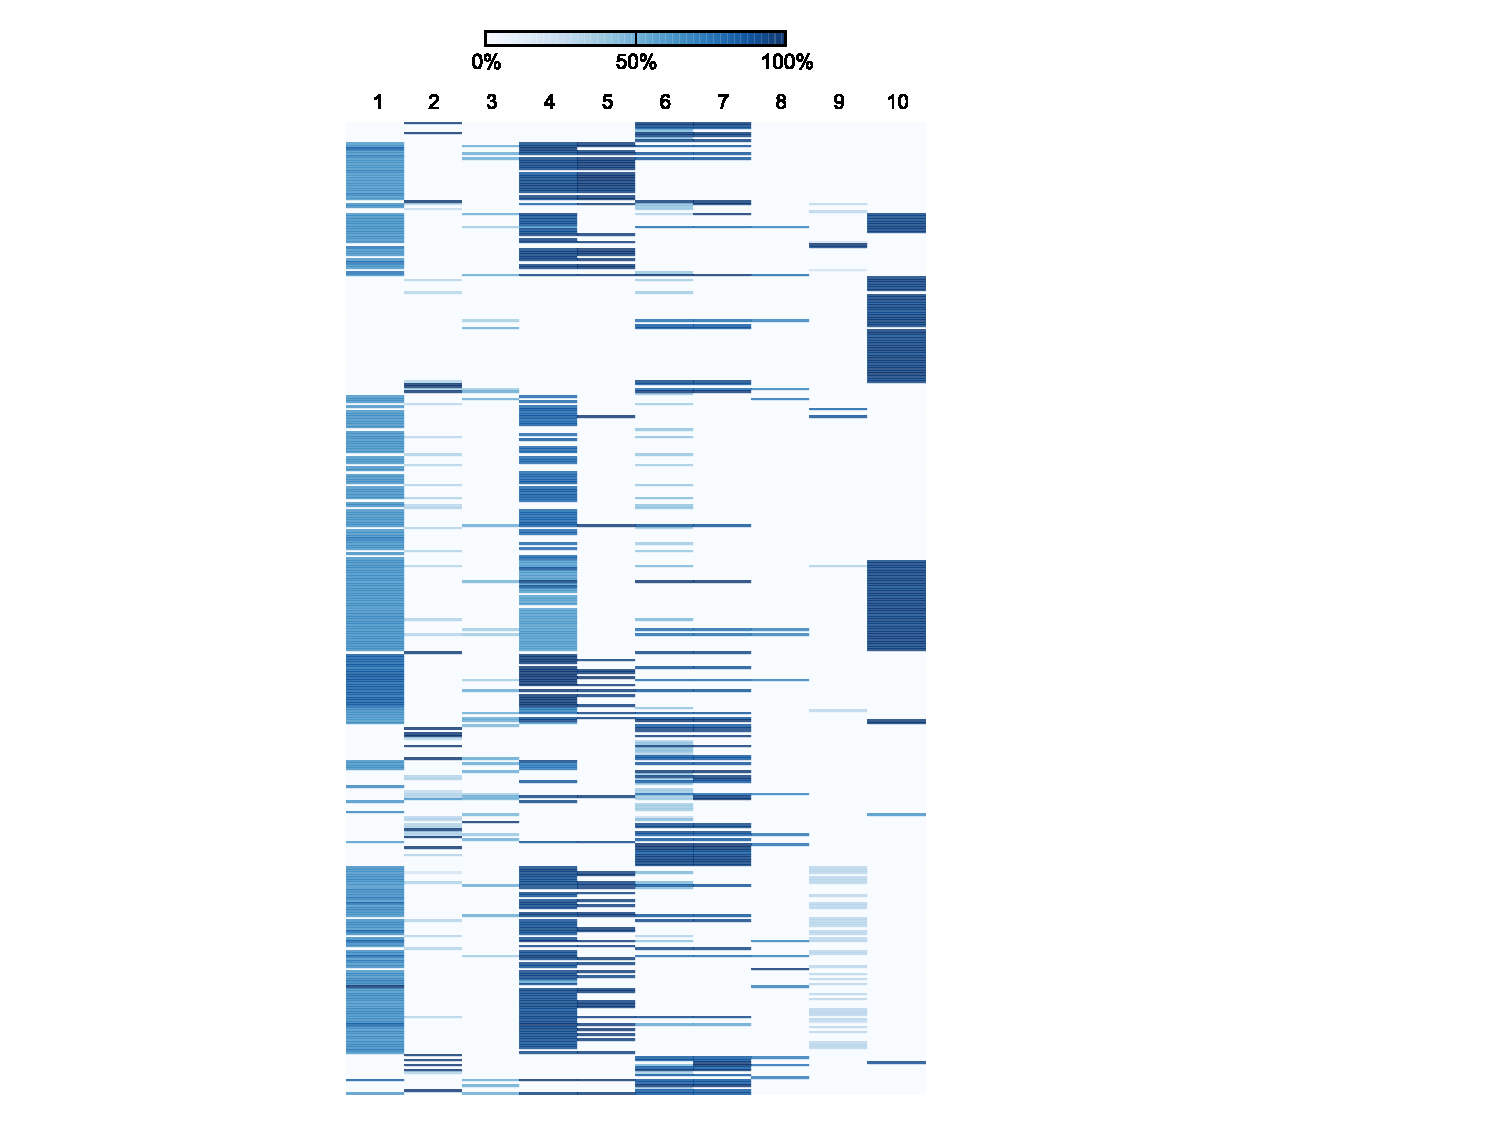
\includegraphics[scale=1.0]{figures/sequence_plot.pdf}}
\caption{Data coverage for a sequence matrix with 10 genes, 384 OTUs, taxon coverage density of 0.26, and partial decisiveness of 0.31.
White represents missing data, and shades of blue represent sequences present. Longer sequences are dark blue, short sequences
are light blue.} \label{fig:01}
\end{figure}

\begin{figure}[!tpb]
\centerline{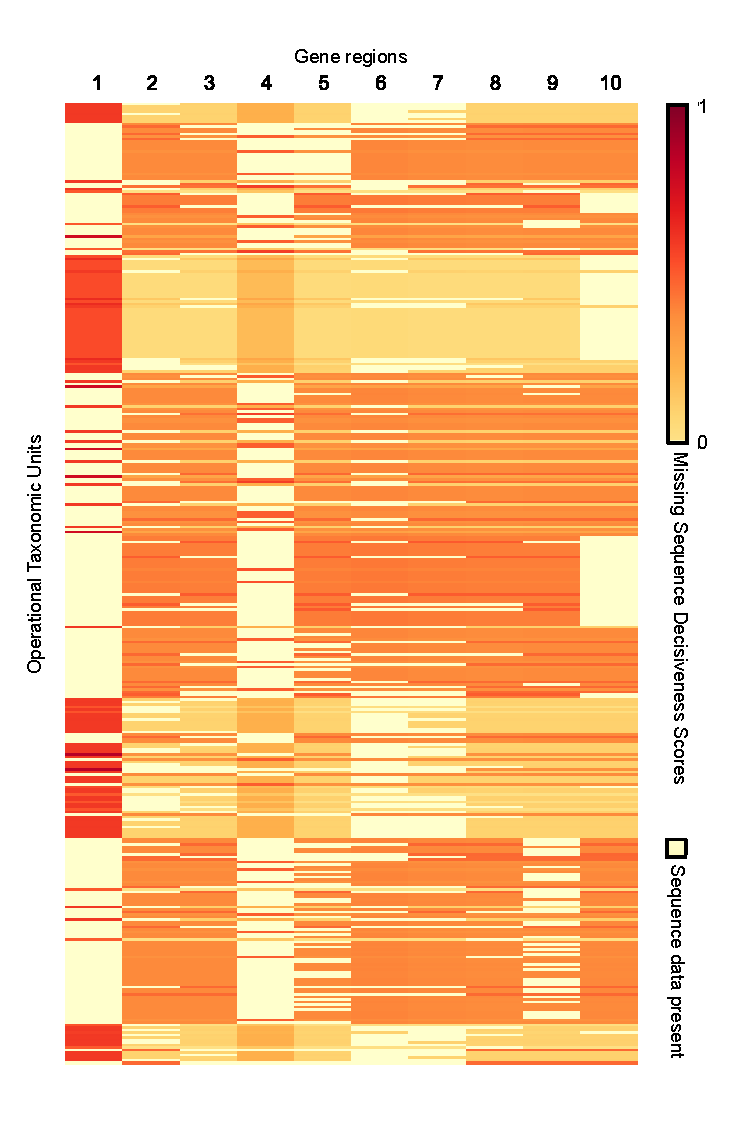
\includegraphics[scale=1.0]{figures/MSDS_figure_1.pdf}}
\caption{Missing Sequence Decisiveness Scores (MSDS) for a sequence matrix with 10 genes, 384 OTUs, taxon coverage density of 0.26, and partial decisiveness of 0.31.
Pale yellow represents sequence data present, shades of orange represent missing sequences with low to intermediate MSDS (~0-0.75),
and red to maroon represents missing sequences with high MSDS (~0.75-1.0).
MSDS measures how much the individual missing sequence contributes to the decisiveness of the matrix given the overall pattern of missing data.
MSDS prioritizes which sequences to add to the matrix; where MSDS is high the addition of new data will increase the
decisiveness of the matrix more than where MSDS is low.}\label{fig:02}
\end{figure}


%\bibliographystyle{natbib}
\cleardoublepage
\phantomsection
\addcontentsline{toc}{chapter}{Bibliography}
\bibliography{SUMAC_manual}

\end{document}
